\documentclass[hidelinks]{article}
\usepackage{graphicx} % Required for inserting images
% Language setting
% Replace `english' with e.g. `spanish' to change the document language
\usepackage[german]{babel}

% Set page size and margins
% Replace `letterpaper' with `a4paper' for UK/EU standard size
%\usepackage[letterpaper,top=2.5cm,bottom=2cm,left=2.5cm,right=2.5cm,marginparwidth=1.75cm]{geometry}
\usepackage[a4paper,top=2cm,bottom=2cm,left=2.5cm,right=2.5cm,marginparwidth=1.75cm]{geometry}

% Useful packages
\usepackage{amsmath,amsthm}
\usepackage{comment}
\usepackage{enumerate}
\usepackage{fancyhdr}
\usepackage{xcolor}
\usepackage{inputenc}
\usepackage{float}
\usepackage[justification=centering]{caption}
\usepackage{csquotes}
\usepackage{tikz}
\usepackage{multicol}
\usepackage{amsmath,amssymb}
\usepackage{wrapfig}
\usepackage{notes2bib}
\PassOptionsToPackage{hyphens}{url}\usepackage{hyperref} % makes urls break
\hypersetup{
    colorlinks=true,
    linkcolor=blue,
    filecolor=magenta,
    urlcolor=cyan,
    pdftitle={Localic Caratheodory Extensions},
    pdfpagemode=FullScreen,
}
\usepackage{svg}
\usepackage{subcaption}

%---------- Lean Syntax Highlighting ----------
\usepackage{fontspec}
% switch to a monospace font supporting more Unicode characters
% \setmonofont{FreeMono}
\setmonofont{JetBrains Mono}
\usepackage{minted}
% instruct minted to use our local theorem.py
\newmintinline[lean]{lean}{bgcolor=white,fontsize=\small}
\newminted[leancode]{lean}{fontsize=\footnotesize,baselinestretch=1.2}
\usemintedstyle{tango}  % a nice, colorful theme


\usepackage[url=true,backend=biber]{biblatex}

% Command for marking things as leanok
\definecolor{darkgreen}{HTML}{1F8F1F}

\setcounter{biburllcpenalty}{7000}
\setcounter{biburlucpenalty}{8000}
\addbibresource{main.bib}


% Define the custom lean citation command.
% When you write \leanok{Example-Declaration} it will:
%   - Print in text a green clickable citation [lean: Example-Declaration]
%     that jumps to the corresponding lean entry.
%   - Append an entry to the lean declarations list containing the key and a URL✔✔✔
%     constructed from the argument.
\newcommand{\hash}{\#}

% Macro to hold the list of lean keys already added
\newcommand{\leankeys}{}

% Macro to hold the lean entries for the Lean-Declarations bibliography
\newcommand{\leanentries}{}

% The custom lean citation command:
\newcommand{\leanok}[1]{%
% Always print the in-text citation (green and hyperlinked)
    \hyperlink{Lean:\detokenize{#1}}{\textcolor{darkgreen}{\textbf{[Lean: #1]}}}%
    % If the key is not already in \lean@keys, then add it and append the entry:
    \ifinlist{#1}{\leankeys}{}{%
        \listgadd{\leankeys}{#1}%
        \gappto{\leanentries}{%
            \item \hypertarget{Lean:\detokenize{#1}}{} \textbf{#1}\quad\url{https://bergschaf.github.io/Localic-Caratheodory-Extensions/docs/find/\hash doc/#1}%
        }%
    }%
}


% Macro to hold the list of lean keys already added
\newcommand{\mathlibkeys}{}

% Macro to hold the lean entries for the Lean-Declarations bibliography
\newcommand{\mathlibentries}{}

% The custom lean citation command:
\newcommand{\mathlibok}[1]{%
% Always print the in-text citation (green and hyperlinked)
    \hyperlink{Mathlib:\detokenize{#1}}{\textcolor{darkgreen}{\textbf{[Mathlib: #1]}}}%
    % If the key is not already in \lean@keys, then add it and append the entry:
    \ifinlist{#1}{\mathlibkeys}{}{%
        \listgadd{\mathlibkeys}{#1}%
        \gappto{\mathlibentries}{%
            \item \hypertarget{Mathlib:\detokenize{#1}}{} \textbf{#1}\quad\url{https://leanprover-community.github.io/mathlib4_docs/find/\hash doc/#1}%
        }%
    }%
}

% Macro to hold the list of lean keys already added
\newcommand{\prkeys}{}

% Macro to hold the lean entries for the Lean-Declarations bibliography
\newcommand{\prentries}{}

% The custom lean citation command:
\newcommand{\prok}[1]{%
% Always print the in-text citation (green and hyperlinked)
    \hyperlink{pr:\detokenize{#1}}{\textcolor{blue}{\textbf{[\##1]}}}%
    % If the key is not already in \lean@keys, then add it and append the entry:
    \ifinlist{#1}{\prkeys}{}{%
        \listgadd{\prkeys}{#1}%
        \gappto{\prentries}{%
            \item \hypertarget{pr:\detokenize{#1}}{} \textbf{#1}\quad\url{https://github.com/leanprover-community/mathlib4/pull/#1}%
        }%
    }%
}


%%%%%%%

\title{Langfassung JUFO 2025}
\author{Chiara Cimino}
\date{December 2024}



\title{Lean-Banach Tarski}
\author{Christian Krause, Chiara Cimino}
\newtheorem{satz}{Satz}
\newtheorem{lemma}[satz]{Lemma}
\newtheorem{aussage}[satz]{Aussage}
\newtheorem{korollar}[satz]{Corollary}
\newtheorem{definition}[satz]{Definition}
\newtheorem{bemerkung}[satz]{Bemerkung}
\newtheorem{proposition}[satz]{Proposition}
\newtheorem{example}[satz]{Beispiel}
\newtheorem{notation}[satz]{Notation}
\newtheorem{uberblick}[satz]{Overview}
\newtheorem{vermutung}[satz]{Conjecture}
\newcommand{\rot}[1]{\textcolor{red}{{#1}}}
\newcommand{\blau}[1]{\textcolor{blue}{{#1}}}
\newcommand{\grun}[1]{\textcolor{green}{{#1}}}
\newcommand{\gelb}[1]{\textcolor{yellow}{{#1}}}


% Zeilenabstand
\usepackage{setspace}
\setstretch{1.5}

% Kürzen
\expandafter\def\expandafter\normalsize\expandafter{%
    \normalsize%
    \setlength\abovedisplayskip{0pt}%
    \setlength\belowdisplayskip{8pt}%
    \setlength\abovedisplayshortskip{-8pt}%
    \setlength\belowdisplayshortskip{2pt}%
}
\usepackage{enumitem}
\setlist{nosep}
\setlist{itemsep=0pt}

\pagestyle{fancy}

\begin{document}

    \setlength\parindent{0pt}

    \fancyhf{}

    \rfoot{Chiara Cimino, Christian Krause}

    \lfoot{Jugend forscht 2025}

    \cfoot{Seite \thepage}

    \renewcommand{\headrulewidth}{0pt}

    \renewcommand{\footrulewidth}{0.1pt}



    \raisebox{4.4cm}{\begin{minipage}{0.5\textwidth}

                         
\includegraphics[scale=0.5]{Logo SfZ.png}

    \end{minipage}

        \hspace{4cm}

        \begin{minipage}{0.5\textwidth}

            
\includegraphics[scale=0.5]{Logo Jugend forscht.png}

% \includegraphics[scale=0.36]{OIP.jpg}

        \end{minipage}}

    \thispagestyle{empty}

    \begin{center}

        \vspace{-3.1cm}

        \textbf{\Huge{\sc Jugend forscht 2025}}\\

        \vspace{1.4cm}

        \textbf{\Huge{LEAN, Logik, Lokale:}}
        \vspace{0.2 cm}

        \textbf{\Huge{Banach-Tarski im Licht moderner}}
        \vspace{0.3 cm}

        \textbf{\Huge{Mathematik!}}

        \vspace{0.5 cm}



        \vspace{0.4 cm}

    \end{center}





    \vspace{-0.4cm}
    \begin{figure*}[ht]

        \centering

        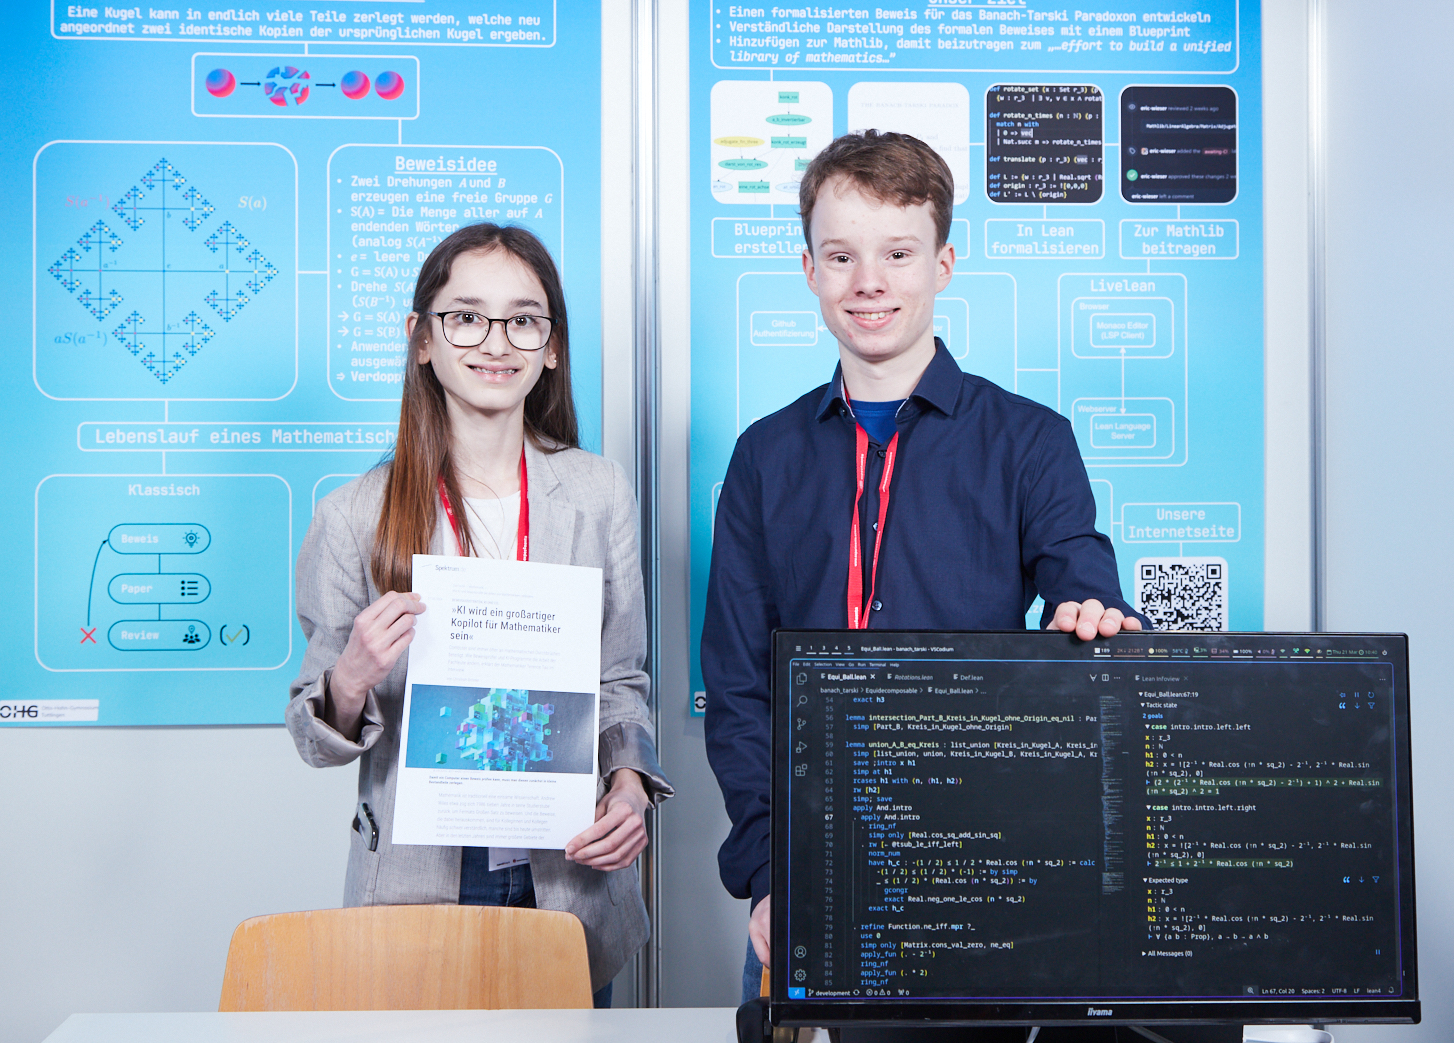
\includegraphics[scale=0.5]{M-07.jpg}

    \end{figure*}
    \begin{center}


        \Large\textsc{Chiara Cimino, Otto-Hahn-Gymnasium Tuttlingen\\Christian Krause, Gymnasium Ochsenhausen}\\\vspace{0.7cm}

        Schülerforschungszentrum Südwürttemberg e.V.\\Standorte Tuttlingen und Ochsenhausen  \vspace{1cm}

        \today

    \end{center}~
    \clearpage
    Das Ziel unseres Jugend-forscht-Projekts des letzten Jahres war es, das Banach-Tarski-Paradoxon, welches besagt, dass wir eine Kugel allein durch Zerlegen und Neuanordnen in zwei identische Kugeln duplizieren können, mithilfe des Beweisassistenten Lean zu formalisieren und der Lean-Community zur Verfügung zu stellen. Aber warum ist diese Art der Kugelverdopplung, die ja offensichtlich den Gesetzen der Physik widerspricht, in der Mathematik überhaupt möglich? Wir machten es uns vor dem Hintergrund dieser Frage deshalb zur Aufgabe, die Problematik hinter Banach-Tarski zu beheben und damit das Paradoxon aufzulösen. Da unsere Arbeit über die Jugend-forscht-Phase hinausging, erreichte uns in einem von zahlreichen Gesprächen mit Mathematikern der Hinweis von Fields Medaillen Träger Laurent Lafforgue auf das französische Manuskript von Olivier Leroy \glqq Les intersections cachees dans le paradoxe de Banach-Tarski\grqq. Dieses Manuskript weist auf eine allgemeinere Theorie hin, in der die Problematik hinter Banach-Tarski behoben wird, weshalb wir uns intensiv mit Leroys Arbeit beschäftigten. Da diese nie in einem Journal veröffentlicht und damit auch nie offiziell geprüft wurde, begannen wir, seine Ideen mit anderen Theorien in Verbindung zu setzen und damit das Manuskript zu vervollständigen. Hierfür mussten wir zunächst einige mathematische Definitionen und Lemmata leanen, wobei es uns bereits gelang, einen signifikanten Teil der Lean-Community zur Verfügung zu stellen. Ausgehend davon formalisierten wir ebenfalls einen beachtenswerten Teil von Leroys Manuskript, arbeiten aktuell an der Fertigstellung und gehen davon aus, diese demnächst abschließen zu können. Mit Leroys Ansatz ist dann der Satz von Banach-Tarski kein Paradoxon mehr, da mit dieser Theorie die Banach-Tarski-Zerlegung nicht mehr disjunkt wäre.

    \section*{Projektübersicht}


    \thispagestyle{empty}

    \clearpage
    \tableofcontents
    \listoffigures
    \thispagestyle{empty}

    \clearpage
    \setcounter{page}{1}


    \section{Fachliche Kurzfassung}
    % Als wir letztes Jahr dabei waren, den Satz von Banach-Tarski in Lean zu formalisieren, sind wir an die Grenzen der klassischen Maßtheorie gestoßen. Der Satz von Banach-Tarski besagt nämlich, dass es theoretisch möglich ist, eine Kugel allein durch Zerschneiden und Drehen zu verdoppeln. Das ist möglich, da während des Zerschneidungsprozesses nicht messbare Teilmengen des topologischen Raums erzeugt werden. Auf der Suche nach einer Lösung für dieses Problem sind wir auf ein nie formal veröffentlichtes Manuskript von Olivier Leroy gestoßen, das verspricht das Problem der nicht messbaren Mengen von Banach-Tarski in der Theorie der Lokalen zu lösen. Dabei werden Unterlokalen anstatt von Teilmengen von topologischen Räumen verwendet. Wir haben es uns zur Aufgabe gemacht, die Grundlagen der Lokalen-Theorie und das von Leroy postulierte Maß zu verstehen und in Lean zu verifizieren. Dafür haben wir bereits viele elementare topologische Definitionen (z.B. Inklusion, Schnitt, Vereinigung und Komplement) auf die Unterlokalen übertragen und in Lean formalisiert. Ausgehend davon arbeiten wir daran, zu zeigen, dass die Caratheodory Erweiterung eines Maßes der offenen Unterlokalen auf alle Unterlokalen einige wichtige maßtheorethische Eigenschaften erfüllt. Damit ist der Satz von Banach-Tarski dann kein Paradoxon mehr, da mit dieser neuen Maßtheorie das Verdoppeln einer Kugel in zwei identische Teile nicht mehr möglich ist.
    Wenn man in der klassischen Maßtheorie ein Maß mithilfe der Caratheodory-Erweiterung erweitert, so besitzt diese Erweiterung im Allgemeinen nicht mehr dieselben nützlichen Eigenschaften wie bspw. die strikte Additivität. Die Folgen sind im Banach-Tarski-Paradoxon zu erkennen, welches eine Kugelverdopplung ermöglicht. Im Zuge dieses Projektes beschäftigen wir uns mit einer Theorie, bei der solche Kuriositäten ohne eine Einschränkung auf die zu messenden Mengen nicht mehr möglich ist und die insbesondere nie in einem mathematischen Journal veröffentlicht wurde. Es handelt sich dabei um die Theorie der Lokale, die Olivier Leroy in seinen Notizen beschrieb. Lokale sind dabei intuitiv als topologische Räume zu verstehen, wobei wir nicht mehr fordern, dass das zugrundeliegende geordnete Mengensystem eine Teilmenge einer gegebenen Menge ist. Daraus resultieren neue Definitionen von Konzepten wie der Vereinigung, dem Schnitt und der Teilmenge im allgemeinen Sinne. Damit lässt sich dann ebenfalls eine Maßtheorie konstruieren, wobei man ein Maß über Lokale ähnlich wie ein klassisches Maß verstehen kann. Betrachtet man allerdings die Caratheodory-Erweiterung eines Maßes über Lokale, so erhält man zusätzlich zu den Eigenschaften der Caratheodory-Erweiterung im klassischen Sinne u. a. eine Reduzibilität und eine strikte Additivität. Daher erhält man eine bessere Maßtheorie! Da dieses unglaubliche Resultat aber nie formal veröffentlicht und damit peer-reviewed wurde, besteht unsere Arbeit darin, genau das zu tun. Hierfür verwenden wir den mathematischen Beweisassistenten Lean, mit dessen Hilfe wir Ungenauigkeiten und Fehler im Beweis von Leroy aufdecken und beheben konnten und damit den Großteil seiner Theorie bereits in Lean formalisiert haben. Des Weiteren gelang es uns bereits, Teile des von uns formalisierten Beweises der Lean-Community zur Verfügung zu stellen. Bereits in Lean formalisierte mathematische Theoreme werden in einer allgemein zugänglichen Bibliothek, genannt Mathlib, gespeichert.


    \section{Motivation und Aufgabenstellung}
    \glqq Wir können eine Kugel allein durch Zerschneiden und anschließendem Drehen wieder zu zwei identischen Kopien der Ausgangskugel zusammenfügen.\grqq~Dass das mit der klassischen Mengenlehre gilt, folgt aus dem Satz von Banach-Tarski \autocite{noauthor_banach-tarski-paradoxon_2024}. Auch uns erschien diese Aussage anfänglich unglaublich, weshalb wir in unserem Jugend-forscht-Projekt des letzten Jahres den mathematischen Beweis des Banach-Tarski-Paradoxons näher beleuchteten. Indem wir den Beweis Stück für Stück durchdrangen, gingen wir automatisch den Weg einer klassischen Verifikation eines mathematischen Papers (siehe Abbildung \ref{Abb1}, linke Spalte). Da der Prozess der menschlichen Kontrolle aber durchaus fehleranfällig ist, stellten wir uns die Frage, ob man diese Fehlbarkeit nicht umgehen könnte. Dabei stießen wir auf den mathematischen Beweisassistenten Lean. Diese auf der gleichnamigen Programmiersprache Lean basierende Software erlaubt es uns, die entsprechenden mathematischen Objekte zu definieren, sowie deren Eigenschaften inkl. Beweis zu formalisieren. Ausgehend von der Typentheorie überprüft Lean die Standhaftigkeit des Beweises und markiert ggf. Fehler, was das Beweisen erleichtert. Dies bedeutet im Umkehrschluss aber auch, dass Lean den Anspruch einer absoluten mathematischen Korrektheit erheben kann (siehe Abbildung \ref{Abb1}, rechte Spalte). Die Lean Community, zu der wir nun seit einem Jahr gehören, hat bereits über die Hälfte des Grundstudiums der Mathematik, sowie einige sehr fortgeschrittene Konzepte in insgesamt über eine Million Zeilen Code digitalisiert.

    \begin{minipage}{.38\textwidth}
        Das ist auch der Grund, weshalb sich Mathematikerinnen und Mathematiker weltweit vernetzen, um weitere Sätze in Lean zu formalisieren. Hier erleben wir eine wunderbare und effektive Zusammenarbeit der Informatik und der Mathematik. \\
    \end{minipage}
    \begin{minipage}{.5\textwidth}
        \begin{center}
            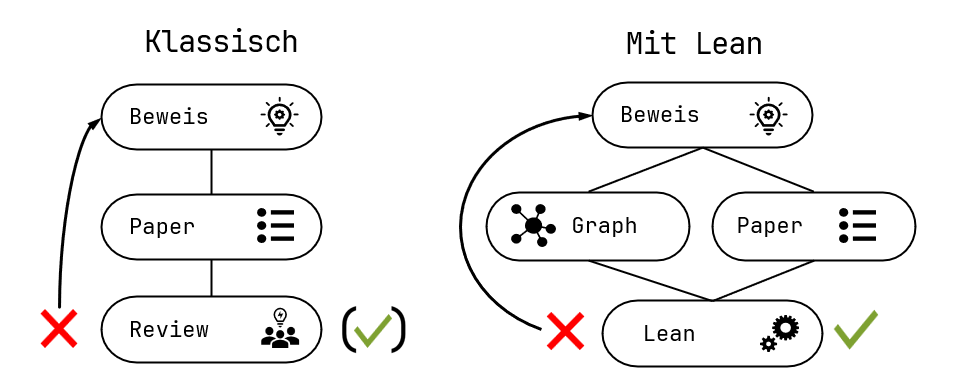
\includegraphics[width=1.3\textwidth]{Formalisierung_Grafik.png}
        \end{center}
        \caption{Verifikation mit bzw. ohne Beweisassistent}
        \label{Abb1}
    \end{minipage}\\

    \noindent Bereits in Lean formalisierte mathematische Theoreme werden in einer allgemein zugänglichen Bibliothek, genannt Mathlib, gespeichert. Die Lean Community, zu der wir nun seit einem Jahr gehören, hat bereits über die Hälfte des Grundstudiums der Mathematik, sowie einige sehr fortgeschrittene Konzepte in insgesamt über eine Million Zeilen Code digitalisiert. Das ist auch der Grund, weshalb sich Mathematikerinnen und Mathematiker weltweit vernetzen, um weitere Sätze in Lean zu formalisieren. Hier erleben wir eine wunderbare und effektive Zusammenarbeit der Informatik und der Mathematik. \\


    \noindent Je länger wir uns jedoch mit dem Beweis des Satzes von Banach-Tarski beschäftigten, desto öfter kam die Frage auf, warum das Duplizieren einer Kugel allein durch Zerlegung der Ausgangskugel sowie anschließender Translationen und Zusammenfügen der einzelnen Teile in der Mathematik überhaupt erlaubt sein sollte, zumal dies der klassischen Physik widerspricht. Ein Ziel der Mathematik ist es, die Vorgänge um uns herum bestmöglich zu beschreiben und damit so gut wie es geht zu verstehen. Ein mathematisches Modell, das es uns erlaubt, in der Theorie Dinge zu tun, die in der Realität aber erwiesenermaßen nicht möglich sind, ist damit unvollständig. Da die Hauptaussage des Satzes von Banach-Tarski darin besteht, dass eine Kugel (insbesondere deren Volumen) verdoppelt werden kann, steht der Satz von Banach-Tarski im Gegensatz zum allgemein gültigen Erhaltungssatz in der Physik, nach dem das Gesamtvolumen nach dem Zerschneiden und Rotieren der Kugelteile zusammen wieder dem Volumen der Ausgangskugel entsprechen sollten. Da dies laut dem Satz von Banach-Tarski aber nicht der Fall ist, beschreibt das zugrundeliegende mathematische Modell des Satzes von Banach-Tarski die Realität nur unzureichend und es stellte sich uns die Frage, ob es nicht ein besseres mathematisches Modell gibt, welches genau solche Schlupflöcher nicht mehr zulässt. Um das aber sauber abgrenzen zu können, ist es essentiell, dass wir das mathematische Modell hinter dem Satz von Banach-Tarski, die klassische Maßtheorie, näher betrachten.


    \section{Kurzer Einblick in die benötigte klassische Maßtheorie}
    Das Grundprinzip der Maßtheorie besteht darin, einer Ansammlung an Mengen eine sinnvolle Größe zuzuordnen. Betrachten wir daher als Einführung ein Beispiel. Gegeben sei die Menge aller Rechtecke. Jedem dieser in der Menge enthaltenen Rechtecke wollen wir nun eine Größe bzw. einen sinnvollen Flächeninhalt zuordnen. Solch eine Größe definiert sich in unserem Beispiel als Produkt aus Länge mal Breite des entsprechenden Rechtecks. Durch diese Zuordnung wird ein sog. Maß definiert. Allgemein versteht man unter einem Maß allerdings folgendes:
    % Die Maßtheorie \autocite{noauthor_mastheorie_2023} entstand aus dem Versuch, eine Maßfunktion zu definieren, die jeder Teilmenge eines Raumes eine sinnvolle Größe (z. B. Flächeninhalt) zuordnet. Betrachtet man daher bspw. die Menge aller Rechtecke, so kann mithilfe eines Maßes jedem Rechteck das Produkt aus Länge mal Breite zugeordnet werden. Fordert man allerdings gleichzeitig $\sigma$-Additivität und Bewegungsinvarianz dieser Maßfunktion, so muss man sich auf eine bestimmte Ansammlung von Mengen beschränken, wie Giuseppe Vitali zeigte. Diese Mengen werden als messbar bezeichnet. Auf ihnen können wir daher sog. Maße definieren:

    \begin{definition}
        Sei $\mathcal{M}$ ein Mengensystem und $\mu:\mathcal{M} \to \overline{\mathbb{R}}$
        eine Abbildung. Man nennt $\mu$ ein Maß, falls folgende Bedingungen erfüllt sind:
        \begin{itemize}
            \item $\mu(\emptyset) = 0$

            \item $\mu(A)$ ist monoton

            \item $\mu$ ist $\sigma$-additiv, insbesondere $\mu(A\cup B)=\mu(A)+\mu(B)-\mu(A\cap B)$ für alle $A, B\in\mathcal{M}$
        \end{itemize}
    \end{definition}
    Wie man erkennen kann, ist ein Maß aber auf ein bestimmtes Mengensystem begrenzt, d. h. Objekte, die nicht in diesem System enthalten sind, kann keine Größe zugeordnet werden. Hat man nun Objekte, die nicht im System vorhanden sind, vorliegen, welche eine ähnliche Struktur wie die Elemente des Systems haben, auf dem unser Maß operiert, so ist es naheliegend sich zu fragen, ob man das vorliegende Maß nicht sinnvoll auf diese Objekte erweitern könnte.

    \begin{minipage}{0.5\textwidth}
        Im Beispiel unseres Maßes, welches jedem Rechteck seinen Flächeninhalt zuordnet, entspräche ein solches zu den Rechtecken ähnliches Objekt zum Beispiel die Fläche des Landkreises Tuttlingen. Um nun der Fläche des Landkreises eine sinnvolle Größe zuzuordnen, können wir diesen zunächst einmal mit Rechtecken überdecken. Für die Überdeckung verwenden wir nun immer kleinere Rechtecke und können so den Flächeninhalt des Landkreises approximieren, indem wir den Grenzwert der Summe der Flächeninhalte dieser kleinen Rechtecke betrachten.
    \end{minipage}
    \begin{minipage}{.5\textwidth}
        \centering
        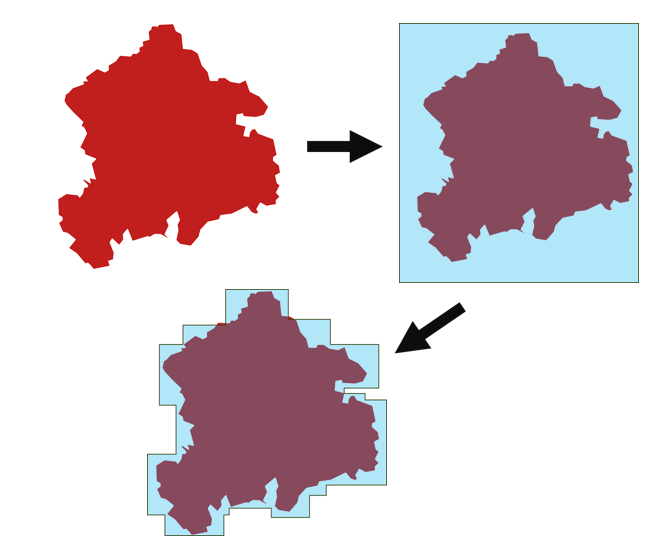
\includegraphics[width=.9\linewidth]{Landkreis approximieren}
        \captionof{figure}{Approximation der Fläche des Landkreises Tuttlingen}
        \label{fig:fläche tut}
    \end{minipage}

    \noindent Diese Approximation von einer zunächst nicht-messbaren Menge mithilfe von messbaren Mengen und einer anschließenden Grenzwertbetrachtung entspricht allgemein genau dem Prinzip der Caratheodory-Erweiterung eines Maßes.


    \begin{definition}
        Sei $\mu$ ein Maß auf einem Mengensystem $\mathcal{M}$. Die Caratheodory-Erweiterung des Maßes ist definiert als
        \[\mu^*(Y)=\inf\{\sum_{i=1}^\infty \mu(A_i)~|~A_i\in\mathcal{M},~Y\subset\bigcup_{i=1}^\infty A_i\}\]
    \end{definition}

    Jetzt haben wir zwar einen sinnvollen Größenbegriff für eine größere Ansammlung an Mengen, jedoch ist zu vermerken, dass bei der Caratheodory-Erweiterung Eigenschaften wie bspw. die allgemeine strikte Additivität verloren gehen. Dieser Verlust der strikten Additivität spiegelt sich bspw. im Banach-Tarski-Paradoxon wider.
    Dass man somit eine Kugel verdoppeln kann, hat uns ziemlich gestört und wir haben uns gefragt, ob es nicht eine Möglichkeit gibt, dass eine Caratheodory-Erweiterung eines Maßes die strikte Additivität des Ausgangsmaßes übernimmt.
    Dabei sind wir auf die Theorie der Lokale gestoßen.


    \section{Die Theorie der Lokale und erste Ergebnisse unserer Arbeit}
    \noindent Unsere Arbeit basiert auf dem Dokument (\glqq Théorie de la mesure dans les lieux réguliers\grqq~(1995) \autocite{leroy_theorie_2013}), das behauptet, dass die Caratheodory-Erweiterung eines Maßen auf die Unterlokalen eines Lokals ein Maß mit guten Eigenschaften (z.B: strikte Additivität) liefert und damit das Banach-Tarski-Paradoxon umgeht.\\
    \noindent Das Problem an diesem Dokument ist allerdings, dass es lediglich aus den Notitzen von Olivier Leroy besteht,
    die nach seinem Tod im Jahr 1996 digitalisiert wurden.
    Daher wurde das Paper auch nie in einem mathematischen Journal veröffentlicht und damit auch nie peer-reviewed (also durch andere Mathematiker kontrolliert).
    Da die Notizen von Leroy zudem teilweise sehr vage formuliert sind, keine Quellenangaben enthalten und mit kleinen
    Fehlern behaftet sind, haben wir es uns zur Aufgabe gemacht, das Paper in Lean zu formalisieren und damit zu
    verifizieren.\\

    \noindent Dafür müssen wir zunächst aber etwas genauer auf die Theorie der Lokale, die eine spezielle Form der
    punktfreien Topologie darstellt, eingehen.
    Ein Lokal \autocite{noauthor_locale_nodate} verhält sich intuitiv wie ein topologischer Raum, der möglicherweise nicht genügend (oder sogar gar keine) Punkte besitzt.
    Stattdessen enthält ein Lokal offene Unterräume. Diese offenen Unterräume können so verstanden werden, dass sie eine
    endliche Menge an Informationen über die (hypothetischen) Punkte beinhalten. Zum Beispiel gibt es ein Lokal aller
    Surjektionen von den natürlichen Zahlen auf die reellen Zahlen. Dieses Lokal hat offensichtlich keine Punkte, da es
    keine derartigen Surjektionen gibt, sie enthält jedoch viele nichttriviale offene Teilräume.
    Leroy zeigt nun durch die Anwendung der Theorie der Lokale, dass es möglich ist, das Auswahlaxiom zu verwenden und dennoch sicherzustellen, dass
    alle \glqq Teilmengen\grqq~messbar bleiben. Dies wird durch die Einführung von Unterlokalen erreicht, die als Unterräume fungieren. In diesem Kontext behauptet er, dass die Caratheodory-Erweiterung eines Maßes auf die Gesamtheit der Unterlokale immernoch strikt additiv, reduzibel und kommutativ bzgl. Infimumbilden ist. Dadurch werden die paradoxen Zerlegungen, wie sie bei Banach-Tarski zu finden sind und die in der klassischen Theorie zu nicht messbaren Mengen führen, in der Theorie der Lokale vermieden, da es versteckte Schnittmengen gibt, die in der klassischen Betrachtung nicht sichtbar sind.\\

    \subsection{Unser Blueprint}
    Ein wesentliches Hilfsmittel, um bei bei der Arbeit in Lean die Übersicht nicht zu verlieren, ist das sogenannte Lean-Blueprint-Tool \autocite{massot_patrickmassotleanblueprint_2025}, das auch in vielen großen Formalisierungsprojekten zum Einsatz kommt.
    Es bietet die Möglichkeit, alle Definitionen und Lemmata für Menschen verständlich zu formulieren und zu dem
    entsprechenden Lean-Code zu verlinken. Eine der wichtigsten Funktionen des Lean-Blueprint-Tools ist wohl der
    interaktive Dependency-Graph (siehe Abbildung \ref{fig:test1}). Dieser stellt alle Beziehungen zwischen den Lemmata und Definitionen übersichtlich in einem Graph dar (also welche Lemmata und Definitionen müssen zuerst fertiggestellt werden). Außerdem kann man anhand der Farbe der Knoten erkennen, wie weit die Formalisierung bereits fortgeschritten ist. \\
    Wir haben für unser Projekt einen solchen Blueprint erstellt, der unter folgender Internetadresse veröffentlicht ist: \url{https://bergschaf.github.io/Localic-Caratheodory-Extensions/blueprint/}.\\
    \begin{figure}[h]
        \centering
        \begin{minipage}{.5\textwidth}
            \centering
            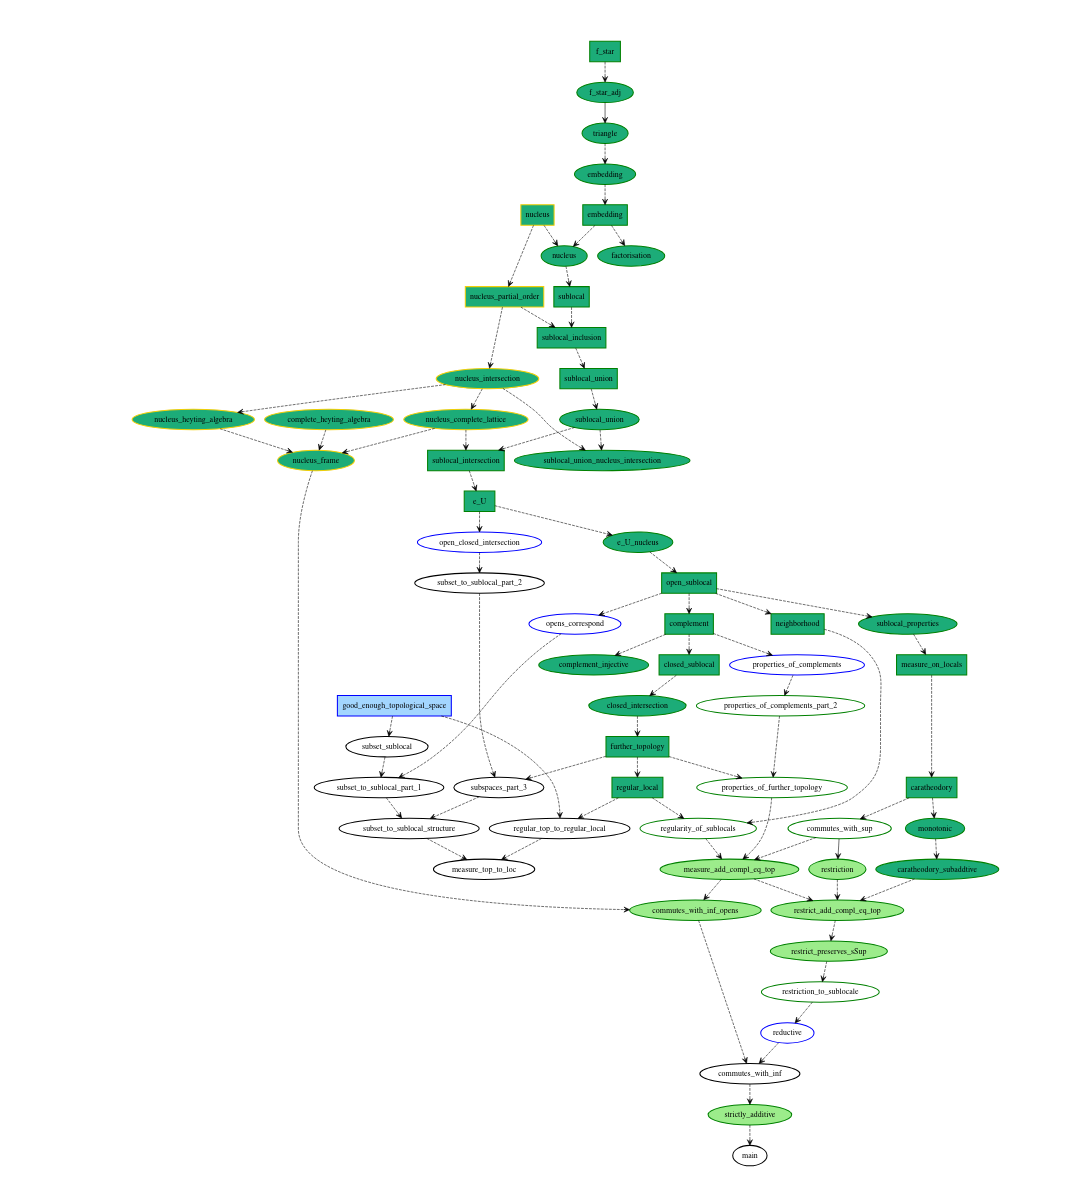
\includegraphics[width=.9\linewidth]{Dependency_Graph_full}
            \captionof{figure}{Gesamtansicht des Blueprints}
            \label{fig:test1}
        \end{minipage}%
        \begin{minipage}{.5\textwidth}
            \centering
            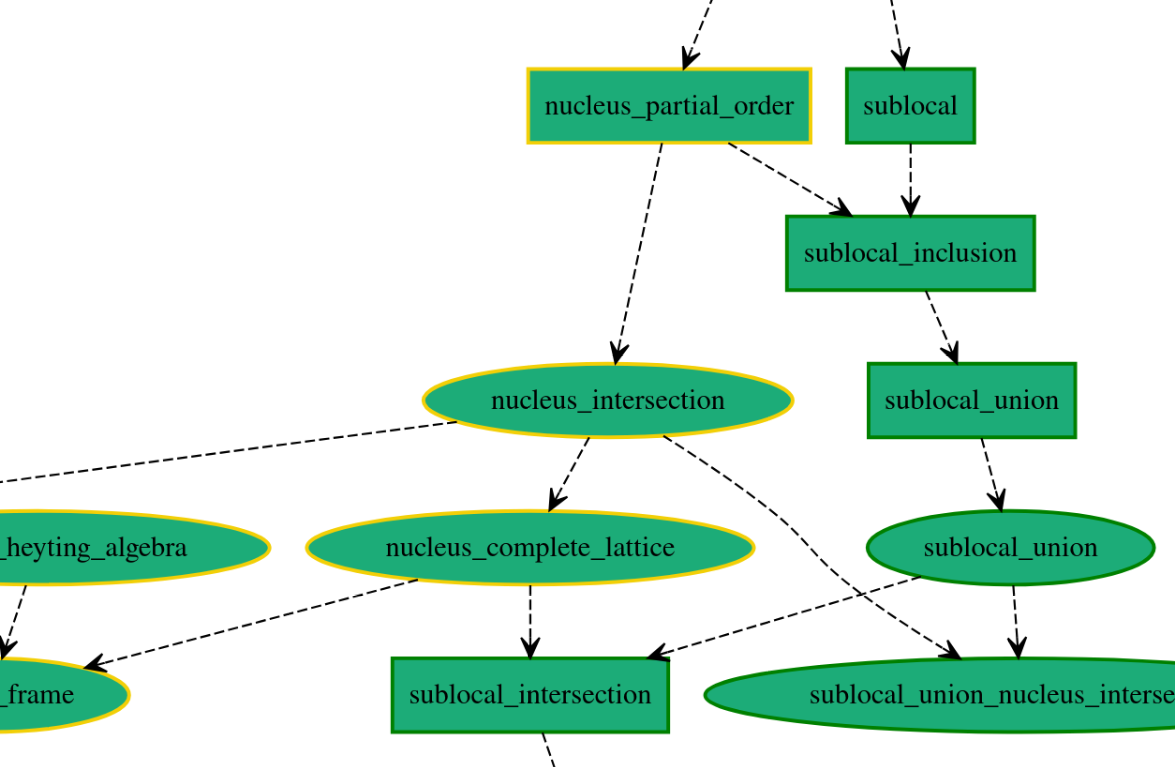
\includegraphics[width=.9\linewidth]{Dependency_Graph_part}
            \captionof{figure}{Ein bereits formalisierter Teil des Blueprints}
            \label{fig:test2}
        \end{minipage}
    \end{figure}
    \clearpage
    \begin{itemize}
        \item Im Blueprint werden Definitionen durch Rechtecke und Lemmata durch Ellipsen dargestellt.
        \item Alles, was bereits fertig formalisiert ist, ist in grün dargestellt.
        \item Eine Definition oder ein Lemma ist blau unterlegt, wenn alle Voraussetzungen bereits formalisiert sind und die Aussage nun bereit für die Formalisierung ist.
        \item Wenn bei einem Lemma nur der Rand eingefärbt ist, bedeutet dies, dass nur die Aussage (nicht aber der Beweis) formalisiert ist (bzw. bereit für die Formalisierung ist).
        \item Ein Klick auf einen Knoten des Graphs öffnet eine Ansicht, die die entsprechende Aussage/Definition anzeigt.
        \item Das Feld \textit{latex} führt zu der ausführlicheren Beschreibung der Aussage bzw. Definition im Fließtext-Teil des Blueprints.
        \item Ist das Lemma oder die Definition bereits fertig formalisiert, dann gelangt man über das Feld \textit{lean} auch zu der automatisch generierten Dokumentation des dazugehörigen Lean-Codes. In dieser Dokumentation ist zu jedem Abschnitt der entsprechende Quellcode unter \textit{source} verlinkt.
    \end{itemize}
    Da wir bereits einen großen Teil unserer Arbeit in Lean verifiziert haben (grüne Knoten), können wir im weiteren Verlauf der Langfassung für viele Lemmata die schriftlichen Beweise weglassen, um für Übersichtlichkeit zu sorgen.
    Die Definitionen und Beweise, die wir in Lean verifiziert haben oder die bereits in der Mathlib enthalten sind, sind folgendermaßen gekennzeichnet:
    \leanok{Measure} bzw. \mathlibok{Nucleus}.
    Die Links zu unserer Lean-Dokumentation bzw. zu der Mathlib-Dokumentation sind im Quellenverzeichniss enthalten.

    \subsection{Elementare Definitionen und Lemmata der Theorie der Lokale}\label{Einführung Lokale}
    Nun wollen wir aber die benötigte Theorie der Lokale besser verstehen. Allgemein besteht ein Lokal $E$ aus einer
    Teilgeordneten Menge $O(E)$ (mit einer Ordnungsrelation $\le$), die die Eigenschaften eines Frames (bzw. einer
    vollständigen Heyting Algebra) erfüllt \mathlibok{Order.Frame}.
    \begin{definition}
        Ein Lokal $E$ besteht aus $(O(E), \le)$, wobei $O(E)$ eine partiell geordnete Menge mit der Ordnungsrelation $\le$
        bezeichnet, die die Eigenschaften eines Frames erfüllt:
        \begin{itemize}
            \item Es existiert ein kleinstes Element $\bot_E$ und ein größtes Element $\top_E$.
            \item Jede Familie $(V_i)$ von Elementen aus $O(E)$ besitzt ein Supremum (genannt Vereinigung), welche mit $\bigvee_i V_i$ bezeichnet wird.
            \item Jede Familie $(V_i)$ von Elementen aus $O(E)$ besitzt ein Infimum (genannt Schnitt), welches mti $\bigwedge_i V_i$ bezeichnet wird.
            \item Für jede Familie $(V_i)$ von Elementen aus $O(E)$ und für ein beliebiges $W\in O(E)$ gilt $W\wedge \bigvee_i V_i = \bigvee_i (W\wedge V_i)$.
        \end{itemize}
    \end{definition}
    Man kann daher erkennen, dass die Definition einer Lokale fast der Definition eines Topologischen Raums entspricht. Der einzige Unterschied besteht dabei darin, dass wir nun nicht mehr fordern, dass das Mengensystem $O(E)$ Teilmenge der Potenzmenge $\mathcal{P}(X)$ einer Ausgangsmenge $X$ ist.
    \begin{example}
        \label{bsp:offeneMengen}
        Die offenen Mengen $O(E)$ eines Topologischen Raumes $E$ bilden mit der Inklusion als Ordnungsrelation ein
        Lokal \mathlibok{TopologicalSpace.Opens.instFrame}.
    \end{example}
    Um irgendeine Operation auf Lokale durchführen zu können, müssen wir zunächst einmal definieren, was wir unter einem Morphismus zwischen zwei Lokale verstehen.
    \begin{definition}
        Seien $E$ und $F$ Lokale. Ein Morphismus $f:E\to F$ wird durch eine monotone Abbildung $f^*:O(F)\to O(E)$ erzeugt, für die gilt:
        \begin{itemize}
            \item $f^*(\bot_F)=\bot_E$ und $f^*(\top_F)=\top_E$
            \item $f^*$ kommutiert mit endlichen Schnitten und beliebigen Vereinigungen
        \end{itemize}
    \end{definition}

    \begin{definition}
        Für jedes $U\in O(E)$ besitzt die Menge der $V\in O(F)$, für die gilt $f^*(V)\subset U$, also ein größtes Element, das wir mit $f_*(U)$ bezeichnen werden.
    \end{definition}

    \begin{lemma}
        Für jeden Morphismus von Lokalen $f:E\to F$ sind die folgenden Eigenschaften äquivalent:
        \begin{itemize}
            \item $f^*$ ist surjektiv
            \item  $f_*$ ist injektiv
            \item $f^* f_*=1_{O(E)}$
        \end{itemize}
        Man nennt einen Morphismus von Lokalen, der diese Eigenschaften erfüllt, Einbettung.
    \end{lemma}
    Eine weitere zentrale Abbildung ist der Nukleus, welchen wir im Folgenden definieren:
    Eine zentrale Abbildung in der Theorie der Lokale ist der Nukleus, den wir im Folgenden definieren:
    \begin{definition}
        \label{def:nukleus}
        Ein Nukleus \autocite[S. 485]{mac_lane_sheaves_1994} ist eine Abbildung $e:O(E)\to O(E)$ mit den folgenden drei Eigenschaften:
        \begin{itemize}
            \item $e$ ist idempotent, d. h. $e\circ e=e$
            \item $U\leq e(U)$ für alle $U\in O(E)$
            \item $e(U\cap V)=e(U)\cap e(V)$ für alle $U,V\in O(E)$
        \end{itemize}
    \end{definition}
    \mathlibok{Nucleus}

    \subsection{Unterlokale}
    Ein wesentliches Konzept der klassischen Topologie sind die Teilengen bzw. Unterräume eines
    Topologischen Raumes, die durch Inklusion geordnet sind. Die Entsprechung in der Theorie der Lokale sind die
    Unterlokale.
    Es gibt mehrere Möglichkeiten, Unterlokale zu definieren \autocite{noauthor_sublocale_nodate}, wir beschäftigen uns hier mit der
    Definition durch Nuklei:
    \begin{definition}
        Ein Unterlokal $X$ eines Lokals $E$ wird durch eine Abbildung $e_X:O(E)\to O(E)$ definiert, die die Eigenschaften eines Nukleus erfüllt (Definition \ref{def:nukleus},Lemma \ref{lemma1}). Folglich ist das von $X$ erzeugte Lokal gegeben durch $O(X)=Im(e_X)=\{V\in O(E) | e_X(V)=V\}$ und die zugehörige Einbettung $i_X:X\to E$ ist durch $i^\ast_X(V)=e_X(V)$, $(i_X)_\ast(U)=U$ definiert. \autocite{noauthor_sublocale_nodate} \leanok{Sublocale}
    \end{definition}

    Die Interaktionen zwischen Unterräumen eines Klassischen Topologischen Raumes (also Inklusion, Vereinigung und
    Schnitt) sind punktweise definiert. Da die Unterlokalen die Unterräume eines klassischen Topologischen Raumes
    in der (Punktfreien) Theorie der Lokalen verallgemeinern, werden diese Interaktionen auf andere Weise definiert.
    Zunächst werden wir zeigen, dass die Nuklei $N(E)$ auf der Lokale $E$ einen Frame \autocite{noauthor_frame_nodate} \mathlibok{Order.Frame} bilden. Da die
    Nuklei direkt mit den Unterlokalen zusammenhängen kann direkt auf die Interaktionen der Unterlokalen geschlossen
    werden.

    \subsubsection{Nuklei als Frame}
    Die Nuklei wurden nicht nur bei Leroy verwendet, daher haben wir uns bei den Folgenden Definitionen auch an Johnstone \autocite{johnstone_stone_1982} und MacLane \autocite{mac_lane_sheaves_1994} orientiert. \\
    Die Ordnungsrelation der Nuklei lässt sich punktweise definieren:
    \begin{definition}
        Für zwei Nuklei $n$ und $m$ gilt $n \le m$, genau dann, wenn $n(V) \leq m(V)$ für alle $V\in O(E)$ gilt.
    \end{definition}
    Die Nuklei bilden damit eine Halbordnung \mathlibok{Nucleus.instPartialOrder}. \\
    Zusätzlich dazu benötigt die Frame Struktur der Nuklei zwei besondere Nuklei; den größten und den kleisten Nukleus:
    \begin{definition}
        Der größte Nukleus $\top_n$ ist definiert durch $\top_n(a)=\top_E$ für alle $a\in O(E)$ \mathlibok{Nucleus.instBot}.\\
        Der kleinste Nukleus $\bot_n$ ist definiert durch $\bot_n(a)= a$ für alle $a \in O(E)$ \mathlibok{Nucleus.instTop}.
    \end{definition}
    $\top_E$ ist das größte Element von $E$ und existiert, da $E$ ein Frame bildet.
    Man sieht direkt, dass der größte Nukleus punktweise größer als alle anderen Nuklei ist.
    Der kleinste Nukleus ist punktweise kleiner als alle anderen Nuklei, da alle Nuklei $x$ die Bedingung $a\le x(a)$ erfüllen müssen. \\
    Bei beliebigen Infima von Nuklei können wir uns an der Definition von Peter Johnstone in seinem Buch \glqq Stone spaces \grqq \autocite{johnstone_stone_1982} orientieren:
    \begin{definition}
        Das Infimum einer Menge $S$ an Nuklei auf $E$ bildet einen Nukleus mit folgender Funktion:
        \[(\bigwedge_n S)(a) = \bigwedge_E \{j(a) \mid j \in S\}\]
        für alle $a \in O(E)$.
    \end{definition}
    Wir haben in Lean verifiziert, dass diese Definition tatsächlich ein Nukleus ist und die Bedingungen eines Infimums erfüllt. \mathlibok{Nucleus.instInfSet} \\
    Suprema von Nuklei lassen sich schwerer mit einer expliziten Formel beschrieben, daher verwenden wir das Infimum aller oberen Schranken:
    \begin{definition}
        Das Supremum einer Menge $S$ an Unterlokalen von $E$ entspricht dem Infimum der oberen Schranken von $S$:
        \[(\bigvee_n S)(a) = (\bigwedge_n \{w \in N(E) \mid x \le w\})(a)\]
        für alle $x \in S$.
    \end{definition}
    Diese Defintion ist ebenfalls ein Nukleus und erfüllt definitionsgemäß die Eigenschaften eines Supremums. \\
    Damit haben wir gezeigt, dass die Nuklei $N(E)$ einer Lokale $E$ einen Vollständigen Verband bilden \mathlibok{Nucleus.instCompleteLattice}.
    Um nun zu zeigen, dass die Nuklei einen Frame bilden, reicht es aus, zu zeigen, dass die Nuklei eine Heyting Algebra \mathlibok{HeytingAlgebra} bilden, da jeder Vollständige Verband, der eine Heyting Algebra ist, einen Frame bildet \mathlibok{Order.Frame}. \\
    \begin{definition}
        Die Heyting Implikation der Nuklei $j$ und $k$ wird durch folgenden Nukleus beschrieben:
        \[(j \Rightarrow k)(a) = \bigwedge \{(j(b) \Rightarrow k(b)) \mid a \le b\})\]
        Für alle $a, b \in E$.
    \end{definition}
    Wir haben in Lean verifiziert, dass diese Definition die Eigenschaften eines Nukleus \mathlibok{Nucleus.instHImp} und die der Heyting Implikation erfüllt, was die Nuklei zu einer Heyting Algebra \mathlibok{Nucleus.instHeytingAlgebra} und damit zu einem Frame macht. \\
    Die Nuklei und deren Frame Struktur haben wir bereits zur Mathlib beigetragen.

    \subsubsection{Schnitt und Vereinigung von Unterlokalen}
    Wir bezeichenen den Nukleus, der mit der Unterlokalen $X$ zusammenhängt $n_X$.
    \begin{definition}
        Die Inklusion zweier Unterlokale $X$ und $Y$ von $E$ lässt sich folgendermaßen definieren:
        \[X \subseteq Y \iff n_Y \le n_X\]
        also $n_Y(V) \le n_X(V)$ für alle $V\in O(E)$ \leanok{Sublocale.le\_iff}.
    \end{definition}
    Die Unterlokale bilden daher eine Duale Ordnung zu den Nuklei. \autocite[S. 51]{johnstone_stone_1982} \autocite{noauthor_categorydual_nodate}
    Dadurch können Resultate auf der einen Ordnung zu der dualen Version auf der anderen Ordnung übertragen werden.
    Um im Folgenden zwischen Unterlokalen und Nuklei zu Unterscheiden bezeichnen wir Nuklei mit $n$ und Unterlokale
    mit $s$ (von engl. Sublocale).
    Das größte Element der Nuklei $\top_n$ ist somit das kleinste Unterlokal $\bot_s$ und umgekehrt ($\bot_n = \top_s$). \\
    Aufgrund der Dualen Ordnung der Nuklei können wir von der Frame-Struktur der Nuklei auf die Coframe Struktur \mathlibok{OrderDual.instCoframe} der Unterlokalen schließen und damit die Interaktionen von Unterlokalen definieren. \\
    Wir wollen uns nun aber noch etwas genauer mit der Definition der Vereinigung von Unterlokalen beschäftigen, da
    sie einen Unterschied zwischen der Arbeit von Johnstone und Leroy darstellt:
    Johnstone hat das Supremum der Unterlokale implizit über das Infimum der Nuklei definiert, Leroy definiert das Supremum hingegen direkt über die Unterlokale:
    \begin{definition}
        Der Schnitt einer Menge $S$ an Unterlokalen von $E$ bildet einen Nukleus mit folgender Funktion:
        $$(\bigcup_s S)(a) = \bigcup \{w \in E | \forall x \in S,w \subseteq x\} $$ für all $a \in E$
    \end{definition}
% TODO Quelle leroy seite 5
    Hier haben wir ebenfalls bereits in Lean verifiziert, dass die Funktion die Bedingungen für einen Nukleus und die Bedingungen des beliebigen Supremums erfüllt. \\

    \begin{lemma}
        Die Definitionen von Johnstone und Leroy \autocite[S. 5]{leroy_theorie_2013} sind äquivalent:
        $$(\bigwedge S) (a) = (\bigcup_s S) (a)$$ für alle Mengen an Nuklei $S$ und für alle $a \in E$ \\
            %TODO hier müsste man eig definieren wie man Unterlokale zu Nuklei konvertiert und umgekehrt
    \end{lemma}
    \begin{proof}
        Da wir verifiziert haben, dass beide Suprema die Bedingungen für beliebige Suprema erfüllen, wissen wir, dass beide eine obere Schranke für $S$ bilden \autocite{noauthor_beschrankte_2021}.
        Wir wissen aber ebenfalls, dass beide Suprema die kleinste obere Schranke bilden, daher haben wir $(\bigwedge_n S) \le (\bigcup_s S)$ und  $(\bigcup_s S) \le (\bigwedge_n S)$, woraus die Gleichheit folgt.
            % TODO lean link
    \end{proof}

    \subsection{Offene und abgeschlossene Unterlokale}
    Wie in der klassischen Topologie gibt es auch in der Theorie der Lokalen offene und geschlossene Unterlokalen.
    Da die offenen Mengen $O(E)$ eines Topologischen Raumes $E$ immer eine Lokale bilden (siehe Beispiel \ref{bsp:offeneMengen}), hängen
    die offenen Unterlokalen mit den Elementen $O(E)$ der Lokale $E$ zusammen und entsprechen damit den offenen Mengen eines klassischen Topologischen Raumes.
    Die Komplemente dieser offenen Unterlokalen (bzw. offenen Mengen) bilden die abgeschlossenen Unterlokalen, die mit den abgeschlossenen Mengen eines Topologischen Raumes zusammenhängen. \\

    Johnstone \autocite[S. 50]{johnstone_stone_1982} und MacLane \autocite[S. 488]{mac_lane_sheaves_1994} definieren beide in ihren Büchern die offenen Unterlokalen folgendermaßen:
    \begin{definition}
        \label{def:open}
        Jedes Element $v$ einer Lokale $E$ erzeugt eine offene Unterlokale von $E$ mit der Funktion:
        $$o_v(a) = v \Rightarrow a$$ für alle $a \in E$ \leanok{Open}. % ($\implies$ symbolisiert die Heyting Implikation)% TODO quelle heyting implication
    \end{definition}
    Johnstone und MacLane verwenden hier $v \Rightarrow a$, die sogenannte Heyting-Implikation (auch relatives-Pseudokomplement)\autocite{noauthor_heyting-algebra_2024,noauthor_heyting_nodate}.
    \begin{definition}
        Die Heyting-Implikation erfüllt die Bedingung $a \le b \Rightarrow c$ genau dann, wenn $a \cap b \le c$ für alle $a$, $b$ und $c$. Eine Heyting Algebra ist ein Verband, bei dem diese Operation für alle Elemente definiert ist.
    \end{definition}
    Die Heyting-Implikation kann hier verwendet werden, da die Elemente einer Lokale einen Frame, also eine vollständige Heyting Algebra bilden.\\
    Anhand dieser Eigenschaften haben wir hier auch in Lean wieder verifiziert, dass es sich bei $o_v$ für alle $v \in E$ um einen Nukleus handelt \autocite{noauthor_leroyopen_sublocales_nodate}. % TODO lean link.

    \begin{lemma}
        \label{lem:himp_eq}
        Die Definition der offenen Unterlokale von Johnstone \ref{def:open} ist äquivalent zu der Definition von Leroy:
        \[o_v(a) = \bigcup \{ W \in E | W \cap V \le a \}\]
    \end{lemma}
    \begin{proof}
        Es genügt hier zu zeigen, dass $v \Rightarrow a$ das größte Element in der Menge $S = \{ W \in E | W \cap V \le a \}$ ist.
        Wir wissen, dass $c \le c \Rightarrow a$ genau dann, wenn $c \cap v \le a$, daher sind alle Elemente $S$ kleiner oder gleich wie $v \Rightarrow a$ \mathlibok{himp\_eq\_sSup}.
    \end{proof}
    Wir können nun anhand einiger Eigenschaften der offenen Unterlokalen (analog zu Leroy \autocite[S. 10]{leroy_theorie_2013}) zeigen, dass die offenen Unterlokalen von $E$ nahezu austauschbar mit ihrem entsprechenden Element von $E$ verwendbar sind. Um den folgenden Teil etwas übersichtlicher darzustellen, verwenden wir die Notation $[V]$ für $o_v$. \\
    Uns ist es gelungen, zu verifizieren, dass $[V] \subseteq [U]$ genau dann, wenn $V \subseteq U$ für alle $u, v \in E$ \leanok{Open.le\_iff}.
    Wir haben außerdem gezeigt, dass die offenen Unterlokalen mit beliebigen Suprema kommutieren \leanok{Open.preserves\_sSup}:
    $$\bigcup_i [V_i] = [\bigcup_i V_i]$$
    Für alle Familien $V_i$ aus Elementen von $E$. \\
    Die offenen Unterlokalen kommutieren zudem mit endlichen Infima \leanok{Open.preserves\_inf}:
    $$[U \cap V] = [U] \cap [V]$$
    für alle $U, V \in E$. Diese Eigenschaften haben wir bereits alle in Lean verifiziert. \\


    Johnstone, MacLane und Leroy definieren die abgeschlossenen Unterlokalen alle ähnlich:
% TODO Definition Closed Sublocals (Mclane 488) (Stonespaces S.50)
    \begin{definition}
        Jedes Element $V \in E$ erzeugt eine geschlossene Unterlokale mit dem Nukleus:
        \[c_v(a) = v \cap a\]
        für alle a.
    \end{definition}
    \leanok{Closed}
    Es lässt sich leicht verifizieren, dass es sich bei $c_v$ um einen Nukleus handelt. Leroy zeigt außerdem, dass es sich bei $c_v$ für alle $v \in E$ um das Komplement von $o_v$ handelt. Dies lässt sich anhand der folgenden Eigenschaften beweisen:
    \begin{lemma}
        \[c_v \cap o_v = \bot_s \text{  und  } c_v \cup o_v = \top_s\]
        für alle $v \in E$. \leanok{Open.inf\_compl\_eq\_bot} \leanok{Open.sup\_compl\_eq\_top}
    \end{lemma}
    Wir können also definieren:
    \begin{definition}
        Das Komplement einer offenen Unterlokale $o_v$ entspricht $o_v^c = c_v$ für alle $v \in E$ \leanok{Open.compl}.
    \end{definition}
    \begin{definition}
        Im Folgenden bezeichnen $O(E)$ und $C(E)$ die Menge der offenen bzw. abgeschlossenen Unterlokalen von $E$
    \end{definition}
    Wir können hier $O(E)$ für die offenen Unterlokalen verwenden, da sie mit den Elementen $O(E)$ eines Lokals übereinstimmen. \\

    Mit diesen Definitionen der offenen und geschlossenen Unterlokalen können wir nun einige klassische topologische Operationen auf den Unterlokalen definieren. Diese werden später oft in verschiedenen Beweisen verwendet.
    \begin{definition}
        Der Abschluss einer Unterlokalen $X$ entspricht der kleinsten geschlossenen Unterlokalen, die $X$ enthält \leanok{Sublocale.closure}:
        \[\overline{X} = \bigcap \{W \in C(E) \mid X \le W \}\]
    \end{definition}
    \begin{definition}
        Das Äußere einer Unterlokalen $X$ entspricht der größten offenen Unterlokalen, die disjunkt zu $X$ ist \leanok{Sublocale.exterior}: \[Ext~X = \bigcap \{W \in O(E) \mid W \cap X = \bot_s \}\]
    \end{definition}

    \begin{definition}
        Die offene Umgebung eines Unterlokals $X$ ist die Menge aller offenen Unterlokalen $V$, für die gilt $X \subseteq V$ \leanok{Sublocale.Open\_Neighbourhood}.
    \end{definition}

    \begin{definition}
        Ein Lokal $E$ heißt regulär, wenn für alle offenen Unterlokale $U$ von $E$ die offenen Unterlokale $V$ von $E$ mit $\overline{V} \subseteq U$ ganz $U$ abdecken \leanok{regular}.
    \end{definition}
    Sei $E$ im Folgenden ein reguläres Lokal.
    \begin{lemma}
        \label{lem:regular_sublocal}
        In einem regulären Lokal entspricht jedes Unterlokal $U$ dem Schnitt der offenen Umgebung von $U$.
    \end{lemma}
    Jetzt haben wir die notwendigen Voraussetzungen definiert und kleinere Lücken geschlossen, um mit der Maßtheorie über Lokalen zu beginnen.


    \section{Maßtheorie über Lokale, weitere Ergebnisse unserer Arbeit}\label{Maßtheorie über Lokale}
%Analog zum Aufbau aus dem Blueprint
    Die Maßtheorie über Lokale bietet einen abstrakten Zugang zur Definition von Maßen, der direkt auf der Struktur offener Mengen bzw. offener Unterlokale basiert, ohne auf Punkte oder klassische Mengenoperationen angewiesen zu sein. Statt einzelner Punkte stehen hier offene Teilstrukturen und deren algebraische Beziehungen im Mittelpunkt. Dieser Ansatz erlaubt es, Maßbegriffe auf einer rein strukturellen Ebene zu formulieren. Entsprechend definieren wir ein Maß über Lokale wie folgt:

    \begin{definition}
        Ein Maß auf einem Lokal $E$ ist eine Abbildung $\mu:O(E)\to \mathbb{R}^{+}$, die für alle Unterlokale $U$ und $V$ von $E$ die folgenden Eigenschaften erfüllt:
        \begin{itemize}
            \item $\mu(\emptyset)=0$
            \item $U\subseteq V\implies\mu(U)\leq\mu(V) $
            \item $\mu(U\cup V)=\mu(U)+\mu(V)-\mu(U\cap V)$
            \item $\mu\left(\bigcup_i V_i\right)=\sup_i\mu(V_i)$ für jede monoton steigende Familie $(V_i)_{i\in\mathbb{N}}$ von Elementen aus $O(E)$. D. h., dass für alle $i,j\in\mathbb{N}$ ein $k\in\mathbb{N}$ gibt mit $V_i\cup V_j\subset V_k$ bzw. $V_i\subset V_k$ und $V_j\subset V_k$.
        \end{itemize}

    \end{definition}
    Analog zu der klassischen Maßtheorie, können wir auch hier eine Erweiterung eines Maßes definieren.

    \begin{definition}
        Sei $E$ ein Lokal und $\mu$ ein Maß über $E$. Sei $A$ ein beliebiges Unterlokal von $E$, also insbesondere nicht unbedingt offen. Dann ist $\mu (A)$ definiert durch $\mu (A):=\inf\{\mu (U)~|~A\subset U, U\in O(E)\}$.
    \end{definition}

    \subsection{Elementare Eigenschaften der Maßtheorie über Lokale}
    Wir haben bereits zu großen Teilen in Lean gezeigt, dass ein Maß über Lokale die Eigenschaften eines klassischen Maßes erfüllt, die da wären:
    \begin{lemma}
        Für jedes Maß $\mu$ mit Caratheodory-Erweiterung über ein Lokal $E$ werden folgende Eigenschaften erfüllt:
        \begin{itemize}
            \item Für alle Unterlokale $A,B$ von $E$ gilt $A\subseteq B\Rightarrow\mu(A)\leq\mu(B)$ (\textbf{Monotonie})
            \item Für offene Unterlokale $U$ von $E$ gilt $\mu(U)+\mu(E\setminus U)=\mu(E)$
            \item Für offene Unterlokale $U$ von $E$ und Unterlokale $A$ von $E$ gilt $\mu(A)=\mu(A\cap U)+\mu(A\cap(E\setminus U))$
            \item Für eine monoton steigende Familie $(V_i)_{i\in\mathbb{N}}$ von offenen Unterlokalen von $E$ gilt: $\mu(\sup_i V_i)=\sup_i\mu(V_i)$
            \item Für eine monoton steigende Familie $(V_i)_{i\in\mathbb{N}}$ von offenen Unterlokalen von $E$ und für ein Unterlokal $A$ von $E$ gilt: $\mu(A\cap\sup_i V_i)=\sup_i\mu(A\cap V_i)$
            \item Für eine monoton fallende Familie $(V_i)_{i\in\mathbb{N}}$ von offenen Unterlokalen von $E$ gilt $\mu(\inf_i V_i)=\inf_i\mu(V_i)$
        \end{itemize}
        Insbesondere gilt für zwei offene Unterlokale $U, V$ von $E$ und einem Unterlokal $A$ von $E$
        \[
            \mu(A\cap(U\cup V))=\mu(A\cap U)+\mu(A\cap V)-\mu(A\cap U\cap V)
        \]
    \end{lemma}
    \noindent Dass wir die grundlegenden Bausteine der klassischen Maßtheorie übertragen können, hat zur Folge, dass auch andere fundamentale Konzepte in der Theorie der Lokale erhalten bleiben. Insbesondere wird es uns dadurch erleichtert, die Theorie der Lokale zu verstehen und bestehendes Wissen aus der klassischen Maßtheorie entsprechend anzupassen.\\
    Um exemplarisch den Prozess des Beweisens einer solchen Eigenschaft zu zeigen, beschäftigen wir uns nun mit der folgenden Eigenschaft. Den Beweis dafür haben wir dabei eigenständig ausgearbeitet.
    \begin{lemma}
        Für alle offenen Unterlokalen $U$ von $E$ gilt:
        $$\mu(U) + \mu(U^c) = \mu(\top_s)$$ % TODO ggf das umformulieren oder die anderen eigenschaften in der Notation anpassen
    \end{lemma}
    \begin{proof}
% TODO leroy quelle
        Sei $V$ die Familie der offenen Umgebungen von $U^c$. Sei $W$ die Familie der äußeren von $V$: $W_i := Ext(V_i)$ für alle $i$. Die Vereinigung von $W$ entspricht $U$, da $\bigcap_i V_i = U$ (siehe Lemma \ref{lem:regular_sublocal}). $W$ ist außerdem monoton filtriert, da $U \cup V$ für alle $U, V \in W$ ein Element bildet, das $U$ und $V$ enthält. $U \cup V$ ist in $W$ enthalten, da endliche Schnitte von offenen Umgebungen auch immer eine offene Umgebung bilden. Da $V$ also unter endlichen Schnitten abgeschlossen ist, sind die äußeren von $V$ (also $W$) unter endlichen Vereinigungen abgeschlossen. Da $W$ also monoton filtriert ist, können wir (aufgrund der Eigenschaften von $\mu$ auf den offenen Unterlokalen) folgende Umformung durchführen: $$\mu(U) = \mu(\bigcup_i W_i) = \sup_i \mu (W_i)$$
        Des Weiteren zeigen wir, dass $\mu(W_i) + \mu(V_i) \le \mu(\top_s)$ für alle $i$. Aufgrund der Definition des äußeren wissen wir, dass $W_i \cap V_i = \bot_s$ und $W_i \cup V_i \le \top_s$. Da $\mu(\bot_s) = 0$ und da $\mu$ monoton ist, können wir zeigen:
        $$\mu(W_i) + \mu(V_i) = \mu(W_i) + \mu(V_i) + \mu(W_i \cap V_i) = \mu(W_i \cup V_i) \le \mu(\top_s)$$ für alle $i$.
        Da $U^c \le V_i$ (also $\mu(U^c) \le \mu (V_i)$) wissen wir: $\mu(W_i) + \mu(U^c) \le \mu(\top_s)$. Da dies für alle $i$ gilt und wir vorher gezeigt haben, dass $\mu(U) = \sup_i \mu (W_i)$, haben wir die eine Richtung gezeigt: $\mu(U) + \mu(U^c) \le \mu(\top_s)$. \\
        Um die andere Richtung der Inklusion zu zeigen, beginnen wir mit der Definition der Caratheodory Erweiterung: $\mu(U^c) = \inf_i \mu(V_i)$. Daher wissen wir, dass $\mu(U^c) + \epsilon > \inf_i \mu(V_i)$ für alle $\epsilon > 0$. Es gibt also für alle $\epsilon > 0$ ein $W \in V_i$, sodass $\mu(U^c) + \epsilon > \mu(w)$. Da $W$ eine offene Umgebung von $U^c$ ist, haben wir: $W \cup U^c \ge \top_s$ und daher: $\mu(W) \cup \mu(U) \ge \mu(\top_s)$. Daraus folgt: $$\mu(\top_s) \le \mu(U) + \mu(U^c) + \mu(\epsilon)$$ Da dies für alle $\epsilon > 0$ gilt, können wir $\mu(\epsilon)$ auch mit $inf \{ \mu(\epsilon) | \epsilon > 0\} = 0$ ersetzen und können damit den Beweis abschließen.
    \end{proof}
    Unsere (nicht verkürzte) Lean Formalisierung dieses Beweises nimmt ungefähr 200 Code-Zeilen ein \autocite{noauthor_leroy_lemme3_nodate}. Am Vergleich zu den vier Zeilen im Originaldokument von Leroy \autocite[S. 25]{leroy_theorie_2013} erkennt man gut, dass es, vor allem in diesem Fall, oft ein signifikanter Aufwand ist, schriftliche Beweise in Lean zu formalisieren. Es ist nämlich nicht nur nötig, den Text in Code zu übersetzen, sondern es müssen oft auch wichtige Teile des Beweises \glqq neu gefunden\grqq{} werden, da sie im Originaldokument nicht enthalten sind. Dafür erhalten wir aber die absolute Sicherheit, dass der Beweis korrekt ist, was den einmaligen Aufwand rechtfertigt.

    \subsection{Neue Eigenschaften der Maßtheorie über Lokale}
    Um den Banach-Tarski-Mengen eine sinnvolle Größe in der Theorie der Lokale zuordnen zu können, braucht es selbstverständlich mehr als nur die auch in klassischen Maßen auffindbaren elementaren Eigenschaften. Aktuell sind wir dabei in Lean zu zeigen, dass ein Maß über Lokale mit Caratheodory-Erweiterung folgende neue Eigenschaften aufweist:
    \begin{lemma}
        Sei $E$ ein Lokal und $\mu$ ein Maß über $E$ mit Caratheodory-Erweiterung. Dann besitzt $\mu$ folgende Eigenschaften:
        \begin{itemize}
            \item Für alle Unterlokale $A, B$ von $E$ gilt $\mu (A\cup B)=\mu (A)+\mu(B)-\mu(A\cap B)$ (\textbf{strikte Additivität})
            \item Für eine Familie $(A_i)_{i\in\mathbb{N}}$ von Unterlokalen von $E$ gilt $\mu (\inf A_i)=\inf\mu (A_i)$ (\textbf{kommutiert mit Infimumbilden})
            \item Sei $A$ ein Unterlokal von $E$. Die Menge $\{A'\subset A~\text{Unterlokal von}~E~|~\mu(A')=\mu(A)\}$ hat ein minimales Element (\textbf{Reduzierbarkeit}).
        \end{itemize}
    \end{lemma}

    \noindent Insbesondere gilt nun die strikte Additivität des Maßes mit Caratheodory-Erweiterung für alle Unterlokale eines gegebenen Lokals. Da jede Teilmenge einer gegebenen Menge ein Unterlokal induziert, lässt sich die strikte Additivität auf diese Teilmengen übertragen. Entsprechend können wir festhalten, dass die Caratheodory-Erweiterung nun bessere Eigenschaften hat, die es zusammen mit der besseren Definition des Schnitts möglich machen, den Banach-Tarski-Mengen eine sinnvolle Größe zuzuordnen und dem \glqq Banach-Tarski-Paradoxon\grqq~seinen paradoxen Charakter entziehen, indem ein Duplizieren einer Kugel im Sinne des Satzes von Banach-Tarski nicht mehr möglich ist.


    \section{Zusammenfassung der Ergebnisse und kritische Betrachtung}
    Ein wichtiger Teil unseres Projektes ist es, die Resultate nicht nur zu verstehen und zu Papier zu bringen, sondern parallel auch in Lean zu formalisieren. Das hat einerseits natürlich den Vorteil, dass Beweise mit Lean automatisch sicher verifiziert werden können. Ein weiterer wichtiger Aspekt, bei dem Lean großes Potenzial hat, ist die Zusammenarbeit zwischen Mathematikern. Hier spielt natürlich auch wieder die Verifizierung eine Rolle, da so vor allem in großen Teams nicht jedes Mitglied alle Beweise verstehen und überprüfen muss. Für unser Projekt war es allerdings von deutlich größerer Bedeutung, dass Lean dem Nutzer die Möglichkeit gibt, Definitionen mit einer formalen Sprache standardisiert zu verfassen und in der Mathlib \autocite{noauthor_leanprover-communitymathlib4_2025}
    zu veröffentlichen. Bei dem Aufnahmeprozess in die Mathlib werden Definitionen zudem ausführlich mit anderen Mitwirkenden der Mathlib diskutiert, was die Möglichkeit für wertvolles Feedback gibt. Da eine sogenannte \glqq Pull Request\grqq{} \autocite{noauthor_how_nodate}
    dadurch (in Abhängigkeit von der Komplexität des hinzugefügten Materials) auch etwas länger dauern kann, haben wir uns vorgenommen, bereits vor dem Ende unseres Projektes erste Definitionen und Resultate in der Mathlib zu veröffentlichen.
    Daher haben wir bereits einige Pull Requests \autocite{noauthor_github_nodate} zu verschiedenen Themen erstellt, die auch schon zur Mathlib hinzugefügt wurden:
    \begin{tabular}{c | p{17cm}}
        \prok{21718} & fix(Order/Nucleus): Remove outdated comment                                                                             \\
        \prok{21560} & feat(Order/Nucleus): nuclei form a frame                                                                                \\
        \prok{21515} & feat(Order/Nucleus): nuclei form a complete lattice                                                                     \\
        \prok{21418} & doc(Order/Heyting/Basic): Coheyting difference is not right adjoint                                                     \\
        \prok{21391} & refactor(Order/CompleteBooleanAlgebra): a complete lattice which is a \newline Heyting Algebra is automatically a frame \\
        \prok{21346} & feat(Order/Nucleus): coe\_mk simp lemma                                                                                 \\
        \prok{20918} & doc(Order/Hom/Lattice): warn against \lean{toFun}                                                                       \\
        \prok{20328} & feat(Order/CompleteBooleanAlgebra): Himp in terms of sSup                                                               \\
        \prok{20246} & feat(Order/CompleteLattice): instances for \newline CompleteSemilatticeInf/CompleteSemilatticeSup for Dual types        \\
        \prok{19440} & feat(Order/Nucleus): Nucleus                                                                                            \\
    \end{tabular} \\
    Man sieht, dass wir einen wichtigen Teil unserer Arbeit; den Nukleus und dessen Frame-Struktur bereits in die Mathlib gebracht haben.
    So kann nun jeder, der die Mathlib benutzt, unsere Definition des Nukleus verwenden.
    In einer anderen Pull Request haben wir die Definition des Frames, die bereits in der Mathlib enthalten war, optimiert.
    Wir konnten zeigen, dass das Axiom der Distributivität, das vorher in der Definition enthalten war, nicht benötigt wurde, da es allein daraus folgt, dass ein vollständiger Verband in Kombination mit einer Heyting Algebra vorliegt. \\
    Neben der Arbeit für die Mathlib haben wir parallel in unserem eigenen Github Repository \autocite{bergschaf_bergschaflocalic-caratheodory-extensions_2025} große Teile der elementaren Lokalen-Theorie formalisiert. Dazu gehört die Definition eines Nukleus, die Ordnungsrelation des Nukleus, beliebige Suprema und Infima und schließlich die Verbandsstruktur der Nuklei. Außerdem haben wir die, zu den Nuklei dualen, Unterlokalen mit den entsprechenden Operationen formalisiert. Auch die offenen Unterlokalen und deren Komplemente, die abgeschlossenen Unterlokalen, haben wir bereits in Lean fertiggestellt. Es ist uns außerdem gelungen bereits erste Definitionen und Lemmata der Maßtheorie auf Lokalen zu formalisieren. Dazu gehört einerseits die Definition eines Maßes auf den offenen Unterlokalen, aber auch schon erste Eigenschaften der Caratheodory Erweiterung dieses Maßes. \\

    Um die Arbeit mit Lean zu veranschaulichen, werden wir nun beispielhaft die Definition eines Nukleus betrachten. In der Mathlib haben wir den Nucleus als Erweiterung eines \lean{InfHom} definiert, diese Definition ist etwas anschaulicher, ändert aber nichts an der Bedeutung. Unter folgendem Link man den Lean-Code auf Live-Lean, einer online Lean Plattform, nachvollziehen: \href{https://live.lean-lang.org/#codez=JYWwDg9gTgLgBAWQIYwBYBtgCMBQpKyIobYB0A8lACYCmUpCEAdhDMzaQEJIDOwAxjgD0AWhE4AKqhpwJATzAyIAMzgA5AK790NYHGZwkcAGJQkIDjhFCcPGFC0wNUGZu00NPOAAoAGnAAuWQUaACoASjgAbQBlGhBgdBQYARoASSZVXwBdOAB3aRccODhREVlpOGUNJn4UgxU4NBkmLR1PUmtipohjGsC4f0AkwkHusrgAQXU2jy9gOdpwVhomGE6bEuBFyBgV+G8ADwHfSKC2PqYfc/6DyMATIh6LuAOxsUnp9084ee/al15gEwAObrbqA/j/PjAnxHIInAZHB7XS4vErjKZudpeMAuHh0ABuNDmmVASFBJRxRIJRIA+oDVIc4HJjqdHv1GYBkoiZkQAvGyUXAucimThRTh8UgoMAkFgdHAAN7+ILyRShAC+0UotHopnMMhywjEOAAooDpgBrLFwc1IJiXJDoLy6JgyC7m+qXLA0exIfioXbwPJ0WhMUhWGyAuy2/gyIIXAAywHNMm8mNmg0i/n8BToNG6/Agsb5aY6yPzhbpTAAVjQ6sBCQByKpwIFwVCBPlYZn8XhEqoAbjgPbxXiBg4LwKghvEGJmXx+IGYbBd4ZwOhAICMJZ4pEXLGXKcuQW3GYGjH37DgR87cm6UDy0XPrHY2TBqygEEMcCwbe6qCQhJtgAjAMRhcj+fJGAEfL0jSNAAI40joyhrOAUC/iU/6AagABMHZXqQlJ4lAhI8JWqhGLgJT3tEqBAbkKBtjh3Q0AcvrwMhMBwYh9K7mATFAA}{livelean}. Während eines Beweises wird auf der rechten Seite der aktuelle Stand angezeigt.
    \begin{leancode}
        /--
The Type of Nuclei on a Frame.
-/
structure Nucleus (X : Type*) [SemilatticeInf X] where
  /-- The function of the nucleus.-/
  toFun : X → X
  /-- A Nucleus is idempotent.-/
  idempotent (x : X) : toFun (toFun x) ≤ toFun x
  /-- A Nucleus is increasing.-/
  increasing (x : X) : x ≤ toFun x
  /-- A Nucleus preserves infima.-/
  preserves_inf (x y : X) : toFun (x ⊓ y) = toFun x ⊓ toFun y
    \end{leancode}
    Wir definieren den Nukleus als \lean{structure}, die Funktion des Nukleus und die notwendigen Bedingungen enthält. Eine \lean{structure} in Lean ist vergleichbar mit structs in C oder mit Klassen in objektorientierten Programmiersprachen wie Python. Die \lean{structure} definiert in Lean den Typ aller Nuklei, der aber vom Typ \lean{X} der Lokale, in der sich der Nukleus befindet, abhängt. \lean{[SemilatticeInf X]} stellt sicher, dass der Typ, von dem der Nukleus abhängt, ein Infimum besitzt und mindestens die Eigenschaften eines Semilattices erfüllt. Wir verwenden den Nukleus aber nur auf Lokalen, d.h. der Typ \lean{X} hat bei uns immer eine Frame Struktur.  \\
    Das erste Feld der \lean{structure} enthält die Funktion des Nukleus, die vom Typ \lean{X → X} sein muss. Das nächste Feld \lean{idempotent} erwartet einen Beweis, der versichert, dass die Funktion idempotent ist. Die nächsten beiden Felder enthalten ebenfalls Beweise für die zwei anderen Eigenschaften des Nukleus. \\
    Nun zeigen wir exemplarisch, dass jeder Nukleus monoton ist:
    \begin{leancode}
        /--
A Nucleus is monotone
-/
lemma Nucleus.monotone (n : Nucleus X) : Monotone n := by
  rw [Monotone]
  intro a b h
  have h1 : a ⊓ b = a := inf_eq_left.mpr h
  have h2 := n.preserves_inf a b
  rw [h1] at h2
  exact left_eq_inf.mp h2
    \end{leancode}
    Wir müssen zeigen, dass $n(a) \le n(b)$, wenn $a \le b$, um den Beweis der Monotonie abzuschließen. Daher wissen wir nun in unserem Lean-Beweis, dass $a \le b$ und müssen zeigen, dass $n(a) \le n(b)$. Zuerst zeigen wir  $a \cap b = a$ in \lean{h2}, mit einem Mathlib Lemma, das besagt, dass $a \cap b = a$, wenn $a \le b$. Nun betrachten wir mit \lean{h2} die dritte Eigenschaft von Nuklei, nämlich, dass Infima erhalten werden: $n(a \cap b) = n(a) \cap n(b)$. In dieser Gleichung ersetzen wir mithilfe von \lean{h1}, $a \cap b$ durch $a$. Zum Schluss verwenden wir die andere Richtung des vorherigen Mathlib Lemmas und zeigen, dass $n(a) \le n(b)$, da $n(a) = n(a) \cap n(b)$. \\
    Dies war nur ein sehr einfaches Beispiel für einen Lean-Beweis, unsere, teilweise deutlich komplexeren Beweise, befinden sich in unserem Github Repository \autocite{bergschaf_bergschaflocalic-caratheodory-extensions_2025}.

    \subsection{Der Zusammenhang von Lokale und Topologischen Räumen}
    Wie wir bereits in Kapitel \ref{Einführung Lokale} festgestellt haben, sind sich Topologische Räume und Lokale sehr ähnlich. Schaut man genauer hin, so kann man erkennen, dass Lokale eine Verallgemeinerung von Topologischen Räumen darstellen. Insbesondere induzieren Unterräume hinreichend guter Räume wie etwa Hausdorff Räume oder kompakte Räume, eine Unterlokale. Man kann zeigen, dass dabei die Ordnung der Unterräume in den induzierten Unterlokalen erhalten bleibt. Daraus resultiert, dass ein Maß auf einem hinreichend guten Topologischen Raum $X$ auch ein Maß auf der entsprechenden Lokale induziert, wobei die klassische Caratheodory-Erweiterung auf $\mathcal{P}(X)$ der Einschränkung der Caratheodory-Erweiterung des Maßes auf der induzierten Lokale entspricht.
    Dieser Zusammenhang zwischen Topologischen Räumen und Lokale ist aber nur nebensächlich, weshalb wir uns zunächst auf die Maßeigenschaften der Maße über Lokale konzentrieren. Entsprechend sind diese Zusammenhänge auch noch nicht in Lean formalisiert worden, weshalb vor allem der linke Teil unseres Blueprints verhältnismäßig weiß ist, d. h. wir diese Lemmata und Definitionen noch nicht in Lean formalisiert haben.


    \section{Ausblick}
    Ein wichtiges Ziel ist es, die Grundlagen der Theorie der Lokalen und schließlich auch die Resultate von Leroy in die Mathlib zu übertragen.

    Da wir dann einen Begriff für das Maß über Lokale haben, könnten wir uns damit beschäftigen, ob auch eine Integrationstheorie über Lokale möglich ist und man könnte betrachten, wie mathematische Standard-Sätze in die Theorie der Lokale übertragen werden können.

    Um die Erkenntnisse aus unserer Arbeit in noch allgemeineren Strukturen betrachten zu können, wäre es zudem eine interessante Möglichkeit, u.a. die von uns in Abschnitt \ref{Maßtheorie über Lokale} beschriebene Maßtheorie über Lokale in die Topostheorie einzubetten, um potentiell bessere und allgemeiner geltende Resultate zu erhalten.


%\section{Rückbezug auf Banach-Tarski}
%Kapitel Open subspaces
    \clearpage


    \section{Unterstützungsleistungen}
    \noindent Ein besonderer Dank gilt unseren Betreuern Noa Bihlmaier, Student an der Universität Tübingen, und Helmut Ruf, Lehrer in Tuttlingen. Durch Sie haben wir überhaupt erst von der Theorie der Lokale erfahren. Während der ganzen Zeit haben sie stets geduldig unsere mathematischen Verständnisfragen beantwortet und durch regelmäßige Feedback-Runden unser Projekt strukturiert.

    \noindent Auch wenn wir aufgrund der Unterschiede unserer Wohnorte viel online gearbeitet haben, haben wir uns immer wieder in den Räumen des SFZ in Tuttlingen getroffen. Wir sind sehr dankbar für diese Möglichkeit.\\
    Besonders motiviert hat uns der dritte Platz und das Feedback von der Jury auf dem Landeswettbewerb 2024, vor allem da wir von Dr. Victoria Schleiß eine Einladung auf den International Congress für Mathematical Software in Durham erhielten.
    Dort hatten wir die Möglichkeit, viele interessante Vorträge, u.a. über Lean, zu hören und mit Mathematikern ins Gespräch zu kommen.
    \clearpage


    \section{Quellen}
    \printbibliography[heading=none]
    \section*{Lean-Quellen}
    \begin{enumerate}[label={}]
        \leanentries
        \mathlibentries
    \end{enumerate}
    \section*{Pull-Requests}
    \begin{enumerate}[label={}]
        \prentries
    \end{enumerate}
\end{document}
